\documentclass[12pt, a4paper]{article}

% ── Pacotes ──────────────────────────────────────────────────────────────────
\usepackage[utf8]{inputenc}
\usepackage[T1]{fontenc}
\usepackage[brazil]{babel}
\usepackage{lmodern}
\usepackage{geometry}
\geometry{margin=2.5cm}
\usepackage{graphicx}
\usepackage{float}
\usepackage{booktabs}
\usepackage{longtable}
\usepackage{array}
\usepackage{multirow}
\usepackage{amsmath}
\usepackage{amssymb}
\usepackage{hyperref}
\hypersetup{colorlinks=true, linkcolor=blue, citecolor=blue, urlcolor=blue}
\usepackage{xcolor}
\usepackage{listings}
\usepackage{caption}
\usepackage{subcaption}
\usepackage{setspace}
\usepackage{indentfirst}
\usepackage{natbib}
\usepackage{microtype}

\onehalfspacing

% ── Configuração de código Python ─────────────────────────────────────────────
\definecolor{codebg}{rgb}{0.97,0.97,0.97}
\definecolor{codecomment}{rgb}{0.4,0.4,0.4}
\definecolor{codestring}{rgb}{0.13,0.54,0.13}
\definecolor{codekw}{rgb}{0.00,0.27,0.80}

\lstdefinestyle{python}{
  language=Python,
  backgroundcolor=\color{codebg},
  commentstyle=\color{codecomment}\itshape,
  keywordstyle=\color{codekw}\bfseries,
  stringstyle=\color{codestring},
  basicstyle=\ttfamily\footnotesize,
  breaklines=true,
  captionpos=b,
  frame=single,
  rulecolor=\color{gray!40},
  numbers=left,
  numberstyle=\tiny\color{gray},
  tabsize=4,
  showstringspaces=false,
}

% ── Metadados ─────────────────────────────────────────────────────────────────
\title{%
  \textbf{Análise de Evasão, Conclusão, Trancamentos e Tempo de Permanência
  no Curso de Sistemas de Informação da EACH-USP (2005--2025)}\\[0.5em]
  \large Estudo quantitativo com análise de sobrevivência e modelagem preditiva
}
\author{
  Programa Unificado de Bolsas (PUB) \\
  Escola de Artes, Ciências e Humanidades \\
  Universidade de São Paulo
}
\date{Abril de 2026}

% ─────────────────────────────────────────────────────────────────────────────
\begin{document}

\maketitle
\tableofcontents
\newpage

% =============================================================================
\section{Introdução}
% =============================================================================

A Escola de Artes, Ciências e Humanidades da Universidade de São Paulo
(EACH-USP) iniciou suas atividades em 2005, adotando um modelo pedagógico
baseado na resolução de problemas e no protagonismo estudantil. Ao longo de
vinte anos, o curso de \textbf{Sistemas de Informação} acumulou um histórico
expressivo de matrículas, formando turmas desde a sua primeira coorte.

A diversificação das formas de ingresso na USP — com a incorporação do
ENEM/SISU como via de entrada a partir de meados da década de 2010 — traz
consigo uma questão relevante para o planejamento acadêmico: \emph{existem
diferenças significativas nos padrões de conclusão, evasão e tempo de
permanência entre estudantes que ingressaram por diferentes meios?}

O presente trabalho tem como objetivo analisar os índices de \textbf{evasão},
\textbf{conclusão}, \textbf{trancamento} e \textbf{tempo médio de permanência}
dos alunos do curso de Sistemas de Informação da EACH-USP no período de 2005 a
2025, tomando a forma de ingresso como variável de controle. A análise emprega
métodos de estatística descritiva, testes de hipóteses não-paramétricos,
análise de sobrevivência e regressão logística.

Os resultados esperados fornecem subsídios para o planejamento acadêmico e
para o desenvolvimento de políticas de permanência estudantil, especialmente
no contexto das ações afirmativas e da ampliação do acesso por meio do ENEM.

% =============================================================================
\section{Revisão de Literatura}
% =============================================================================

A evasão no ensino superior é fenômeno multifatorial e amplamente estudado
\citep{tinto1975, baggi2011}. \citet{tinto1975} propõe um modelo teórico que
relaciona a evasão a fatores institucionais, acadêmicos e sociais, argumentando
que a integração do estudante ao ambiente universitário é determinante para a
permanência. No contexto brasileiro, \citet{silva_filho2007} estimam que a
evasão anual em cursos de graduação presenciais supera 20\%, representando
significativo desperdício de recursos públicos.

Estudos mais recentes apontam que políticas de ações afirmativas e a
diversificação das formas de ingresso — como o Sistema de Seleção Unificada
(SISU) — alteram o perfil dos ingressantes e podem influenciar tanto as taxas
de permanência quanto as de conclusão \citep{felicetti2014, vasconcelos2019}.

A análise de sobrevivência tem sido empregada com crescente frequência no
estudo da evasão universitária, pois permite modelar o \emph{tempo até o
evento} (evasão ou conclusão), incorporando naturalmente os dados censurados
— estudantes que ainda estão cursando \citep{borges2020}. O estimador de
Kaplan-Meier, em particular, permite comparar curvas de sobrevivência entre
grupos sem impor pressupostos sobre a distribuição do tempo.

No âmbito da USP, trabalhos institucionais têm documentado variações
significativas nas taxas de aproveitamento entre formas de ingresso, embora
estudos específicos por unidade e curso ainda sejam escassos.

% =============================================================================
\section{Materiais e Métodos}
% =============================================================================

\subsection{Base de Dados}

A base de dados utilizada neste estudo foi extraída do sistema acadêmico
Júpiter da USP, cedida pela área administrativa da EACH. Contém registros de
\textbf{2.849 alunos} com vínculo encerrado no curso de Sistemas de
Informação, cobrindo o período de fevereiro de 2005 a janeiro de 2025. Alunos
com vínculo ativo (cursando, exterior, não-matriculados) foram excluídos para
garantir que todos os registros analisados possuam desfecho definido.

\subsubsection*{Variáveis da base}

\begin{table}[H]
\centering
\caption{Descrição das variáveis da base de dados}
\label{tab:variaveis}
\begin{tabular}{@{}lll@{}}
\toprule
\textbf{Variável} & \textbf{Tipo} & \textbf{Descrição} \\
\midrule
\texttt{ALUNO}             & ID numérico    & Identificador anônimo do aluno \\
\texttt{STATUS}            & Categórico     & Estado final do vínculo (todos: ENCERRADO) \\
\texttt{CR\_ACUMULADO}     & Numérico       & Total de créditos acumulados \\
\texttt{TIPO\_INGRESSO}    & Categórico     & Forma de ingresso na USP \\
\texttt{DATA\_INGRESSO}    & Data           & Data de início do vínculo \\
\texttt{DATA\_ENCERRAMENTO}& Data           & Data de encerramento do vínculo \\
\texttt{TEMPO\_CURSO}      & Numérico (dias)& Duração do vínculo em dias \\
\texttt{TIPO\_ENCERRAMENTO}& Categórico     & Motivo do encerramento \\
\bottomrule
\end{tabular}
\end{table}

\subsection{Variável Derivada: Desfecho}

A variável \texttt{TIPO\_ENCERRAMENTO} foi recodificada em cinco categorias
de desfecho (Tabela~\ref{tab:desfecho}), com base na natureza da saída do
aluno.

\begin{table}[H]
\centering
\caption{Classificação dos desfechos acadêmicos}
\label{tab:desfecho}
\begin{tabular}{@{}ll@{}}
\toprule
\textbf{Desfecho} & \textbf{Códigos de encerramento incluídos} \\
\midrule
Conclusão            & \texttt{CONCLUSAO} \\
Evasão               & \texttt{ABANDONO\_FREQUENCIA}, \texttt{ABANDONO\_MATRICULA}, \\
                     & \texttt{CANC\_CREDITO}, \texttt{CANC\_VENCIMENTO}, \\
                     & \texttt{DESISTENCIA}, \texttt{TRANCAMENTO} \\
Continua na USP      & \texttt{REINGRESSO}, \texttt{TRANSF\_INT} \\
Saída para outra IES & \texttt{TRANSF\_EXT}, \texttt{CANC\_OUTRA\_IES} \\
Outros               & \texttt{FALECIMENTO}, \texttt{DESCUMPRIMENTO\_PEC\_G} \\
\bottomrule
\end{tabular}
\end{table}

\subsection{Grupos de Ingresso}

A base apresenta oito categorias de \texttt{TIPO\_INGRESSO}. Para as análises
inferenciais (testes de hipóteses e análise de sobrevivência), foram
considerados apenas os grupos com tamanho amostral suficiente:
\textbf{FUVEST} ($n = 2.527$) e \textbf{ENEM\_SISU} ($n = 241$). Os demais
grupos são apresentados nas análises descritivas, mas não integram os testes
estatísticos formais.

Coortes de ingresso a partir de 2022 ($n = 32$) foram excluídas das análises
temporais por não disporem de tempo suficiente de observação.

\subsection{Processamento e Análise}

Todas as análises foram realizadas em \textbf{Python 3.12}, utilizando as
seguintes bibliotecas principais:

\begin{itemize}
  \item \texttt{pandas} e \texttt{openpyxl}: carga e manipulação dos dados;
  \item \texttt{scipy.stats}: testes de hipóteses ($\chi^2$, Mann-Whitney);
  \item \texttt{lifelines}: análise de sobrevivência (Kaplan-Meier, log-rank);
  \item \texttt{scikit-learn}: regressão logística e validação cruzada;
  \item \texttt{matplotlib} e \texttt{seaborn}: visualizações.
\end{itemize}

O tempo de curso foi convertido de dias para \textbf{semestres}
(divisão por 180 dias), facilitando a interpretação.

\subsection{Métodos Estatísticos}

\subsubsection{Estatística Descritiva}
Foram calculadas frequências absolutas e relativas, médias, medianas e desvios
padrão para as variáveis \texttt{TEMPO\_SEMESTRES} e \texttt{CR\_ACUMULADO},
segmentadas por forma de ingresso e desfecho.

\subsubsection{Teste Qui-Quadrado de Independência ($\chi^2$)}
Utilizado para verificar se a proporção de evasão (e de conclusão) difere
significativamente entre FUVEST e ENEM\_SISU. A hipótese nula assume
independência entre forma de ingresso e desfecho:
\[
  H_0: P(\text{Evasão} \mid \text{FUVEST}) = P(\text{Evasão} \mid \text{ENEM\_SISU})
\]

\subsubsection{Teste de Mann-Whitney ($U$)}
Empregado para comparar distribuições de \texttt{TEMPO\_SEMESTRES} e
\texttt{CR\_ACUMULADO} entre grupos. Por ser não-paramétrico, é adequado
para distribuições assimétricas. A hipótese nula é que as distribuições são
idênticas entre os grupos.

\subsubsection{Análise de Sobrevivência — Kaplan-Meier}
A análise de sobrevivência modela o tempo até um evento de interesse — neste
caso, a \textbf{evasão}. O estimador de Kaplan-Meier \citep{kaplan1958}
calcula a probabilidade de o aluno \emph{não ter evadido} até cada ponto no
tempo:
\[
  \hat{S}(t) = \prod_{t_i \leq t} \left(1 - \frac{d_i}{n_i}\right)
\]
onde $d_i$ é o número de evasões no semestre $t_i$ e $n_i$ é o número de
alunos em risco. Alunos que concluíram, transferiram-se ou continuam na USP
são tratados como \textbf{censurados}.

A comparação entre curvas de FUVEST e ENEM\_SISU foi feita com o
\textbf{teste log-rank} \citep{mantel1966}, que testa a hipótese:
\[
  H_0: S_{\text{FUVEST}}(t) = S_{\text{ENEM\_SISU}}(t), \quad \forall t
\]

\subsubsection{Regressão Logística}
Um modelo de regressão logística foi ajustado para estimar a probabilidade de
evasão em função de três preditores: forma de ingresso (ENEM\_SISU = 1,
FUVEST = 0), tempo de curso (semestres) e créditos acumulados. O modelo foi
avaliado por validação cruzada estratificada de 5 dobras, utilizando a
área sob a curva ROC (AUC) como métrica.

O desempenho preditivo foi interpretado com cautela, dado que as variáveis
\texttt{TEMPO\_CURSO} e \texttt{CR\_ACUMULADO} são parcialmente consequência
do desfecho (endogeneidade), sendo o modelo útil sobretudo para quantificar
a direção e magnitude das associações.

% =============================================================================
\section{Resultados}
% =============================================================================

\subsection{Estatísticas Descritivas Gerais}

A base analisada contém 2.849 registros com vínculo encerrado, distribuídos
entre oito formas de ingresso (Tabela~\ref{tab:ingresso_n}). O período de
ingresso abrange de fevereiro de 2005 a janeiro de 2025.

\begin{table}[H]
\centering
\caption{Distribuição por forma de ingresso}
\label{tab:ingresso_n}
\begin{tabular}{@{}lrr@{}}
\toprule
\textbf{Forma de ingresso} & \textbf{n} & \textbf{\%} \\
\midrule
FUVEST           & 2.527 & 88,7 \\
ENEM\_SISU       &   241 &  8,5 \\
TRANSF\_INTERNA  &    45 &  1,6 \\
TRANSF\_EXTERNA  &    25 &  0,9 \\
CONV\_PEC\_G     &     6 &  0,2 \\
GRADUADO         &     2 &  0,1 \\
ENEM\_USP        &     2 &  0,1 \\
OLIMP            &     1 &  0,0 \\
\midrule
\textbf{Total}   & \textbf{2.849} & \textbf{100,0} \\
\bottomrule
\end{tabular}
\end{table}

A distribuição geral dos desfechos evidencia que \textbf{61,5\% dos alunos
concluíram} o curso, enquanto \textbf{31,4\% evadiram} (Tabela~\ref{tab:desfechos_geral}).

\begin{table}[H]
\centering
\caption{Distribuição geral dos desfechos}
\label{tab:desfechos_geral}
\begin{tabular}{@{}lrr@{}}
\toprule
\textbf{Desfecho}            & \textbf{n}     & \textbf{\%}  \\
\midrule
Conclusão                    & 1.751          & 61,5 \\
Evasão                       &   896          & 31,4 \\
Continua na USP              &   191          &  6,7 \\
Saída para outra IES         &     6          &  0,2 \\
Outros                       &     5          &  0,2 \\
\midrule
\textbf{Total}               & \textbf{2.849} & \textbf{100,0} \\
\bottomrule
\end{tabular}
\end{table}

\subsection{Desfechos por Forma de Ingresso}

A Figura~\ref{fig:desfecho_ingresso} apresenta a distribuição dos desfechos
por forma de ingresso. Os grupos FUVEST e ENEM\_SISU apresentam taxas de
conclusão semelhantes (61,6\% e 60,6\%, respectivamente). TRANSF\_EXTERNA
destaca-se com a maior taxa de conclusão (76\%), enquanto TRANSF\_INTERNA
apresenta a maior taxa de evasão (40\%).

\begin{figure}[H]
  \centering
  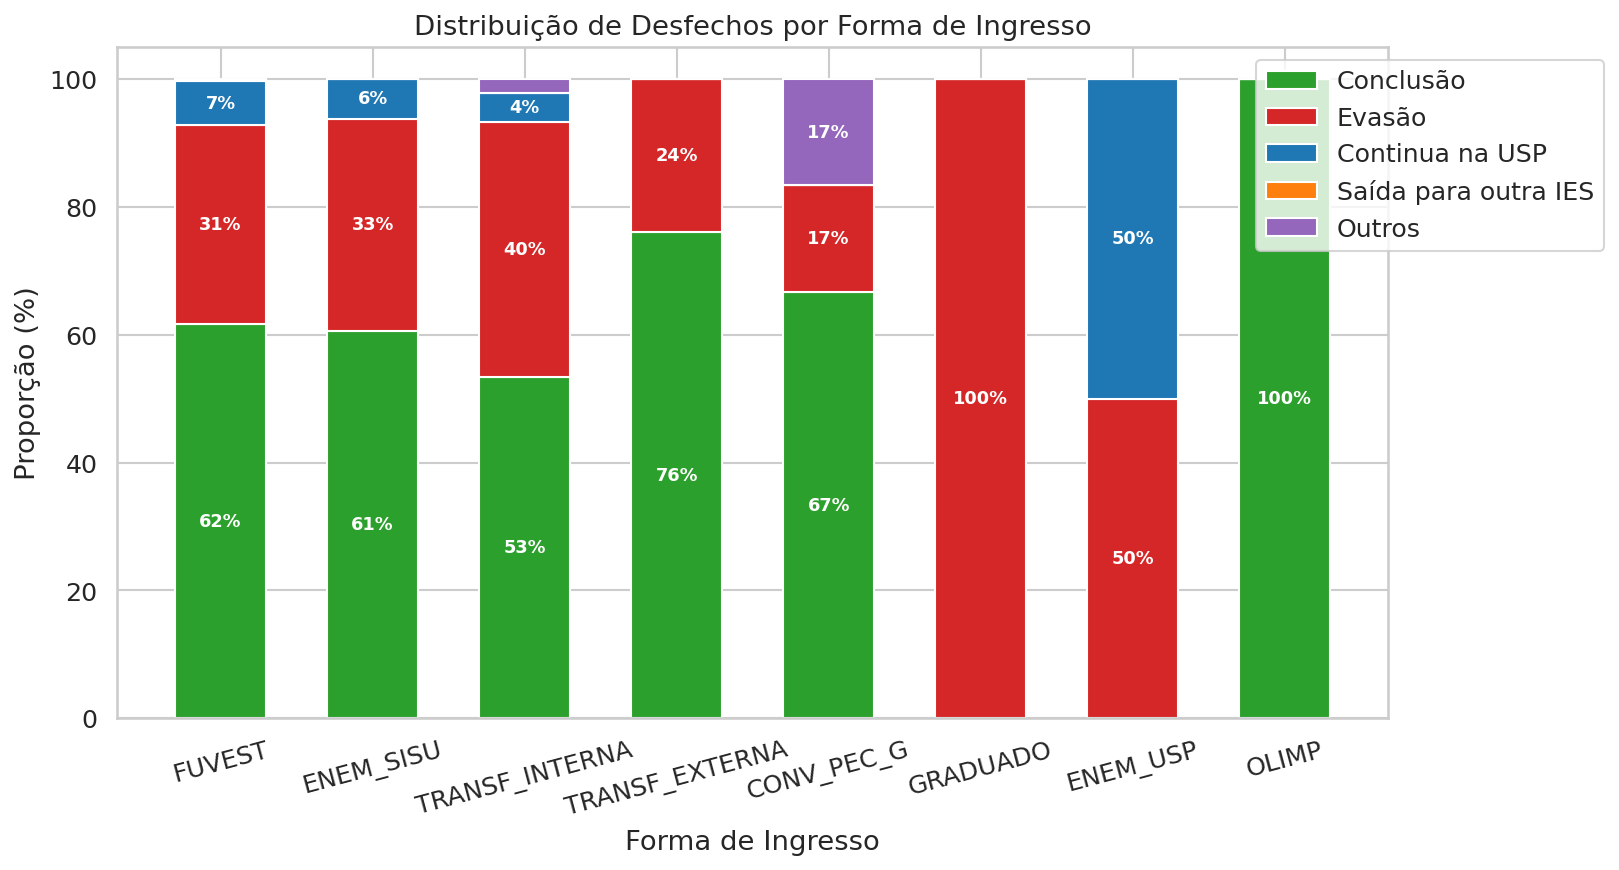
\includegraphics[width=0.92\textwidth]{figuras/fig1_desfecho_por_ingresso.png}
  \caption{Distribuição de desfechos por forma de ingresso. Os percentuais
  são calculados dentro de cada categoria de ingresso.}
  \label{fig:desfecho_ingresso}
\end{figure}

\begin{table}[H]
\centering
\caption{Taxas de conclusão e evasão por forma de ingresso (\%)}
\label{tab:taxa_desfecho}
\begin{tabular}{@{}lrrrr@{}}
\toprule
\textbf{Ingresso} & \textbf{n} & \textbf{Conclusão (\%)} & \textbf{Evasão (\%)} & \textbf{Continua USP (\%)} \\
\midrule
FUVEST           & 2.527 & 61,6 & 31,2 & 6,8 \\
ENEM\_SISU       &   241 & 60,6 & 33,2 & 6,2 \\
TRANSF\_INTERNA  &    45 & 53,3 & 40,0 & 4,4 \\
TRANSF\_EXTERNA  &    25 & 76,0 & 24,0 & 0,0 \\
CONV\_PEC\_G     &     6 & 66,7 & 16,7 & 0,0 \\
\bottomrule
\end{tabular}
\end{table}

\subsection{Motivos de Evasão}

Dos 896 alunos que evadiram, o motivo mais frequente foi o
\textbf{cancelamento por créditos insuficientes} (CANC\_CREDITO), com 386
casos (43,1\%), seguido de \textbf{trancamento sem reingresso} com 202 casos
(22,5\%). A Figura~\ref{fig:motivos_evasao} detalha a distribuição completa.

\begin{figure}[H]
  \centering
  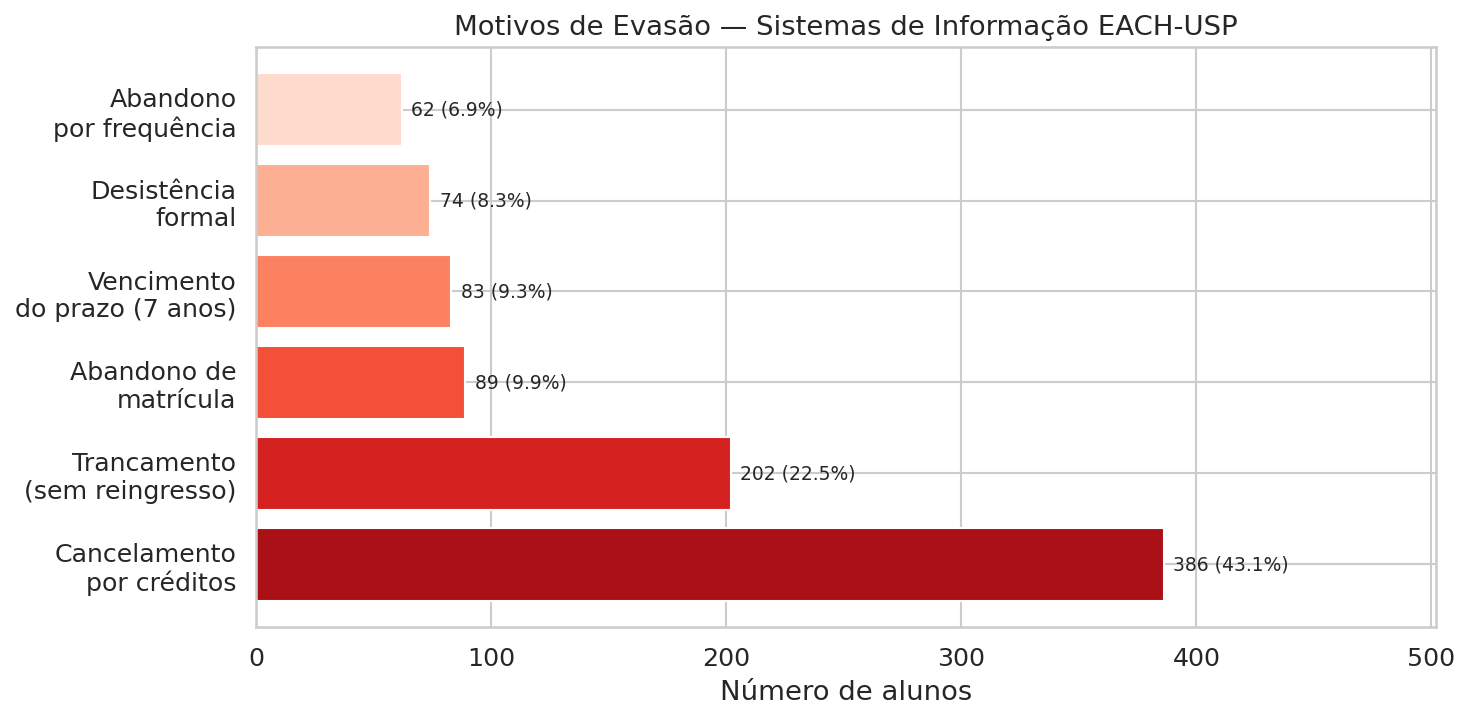
\includegraphics[width=0.90\textwidth]{figuras/fig2_motivos_evasao.png}
  \caption{Distribuição dos motivos de evasão no curso de Sistemas de
  Informação (n=896).}
  \label{fig:motivos_evasao}
\end{figure}

\subsection{Tempo de Curso}

\subsubsection{Tempo de Conclusão}

Alunos que concluíram o curso levaram, em mediana, \textbf{10,2 semestres}
(FUVEST: 10,2 sem; ENEM\_SISU: 9,2 sem). A Figura~\ref{fig:boxplot_tempo}
apresenta a distribuição comparativa, e a Figura~\ref{fig:violin_conclusao}
detalha a densidade do tempo de conclusão por grupo.

\begin{figure}[H]
  \centering
  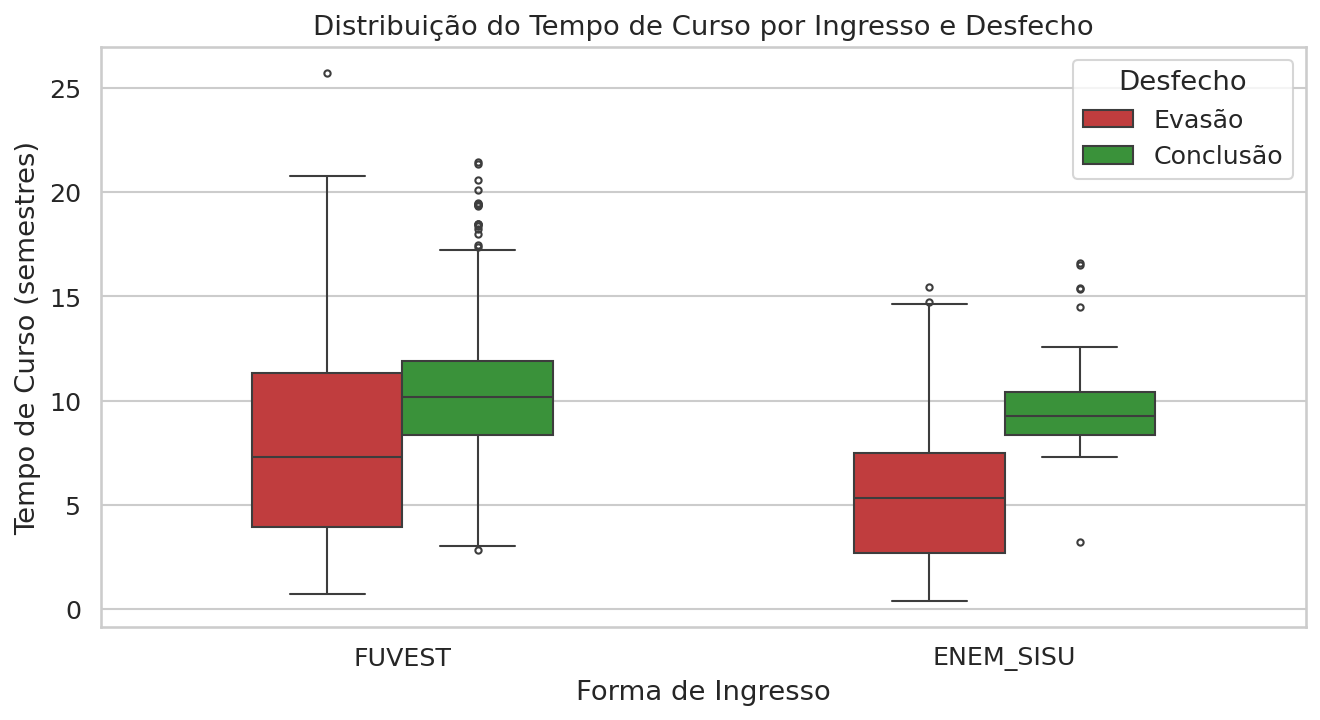
\includegraphics[width=0.85\textwidth]{figuras/fig3_boxplot_tempo.png}
  \caption{Distribuição do tempo de curso (em semestres) por forma de
  ingresso e desfecho. FUVEST: $n_{\text{conc}}=1.557$,
  $n_{\text{ev}}=788$; ENEM\_SISU: $n_{\text{conc}}=146$, $n_{\text{ev}}=80$.}
  \label{fig:boxplot_tempo}
\end{figure}

\begin{figure}[H]
  \centering
  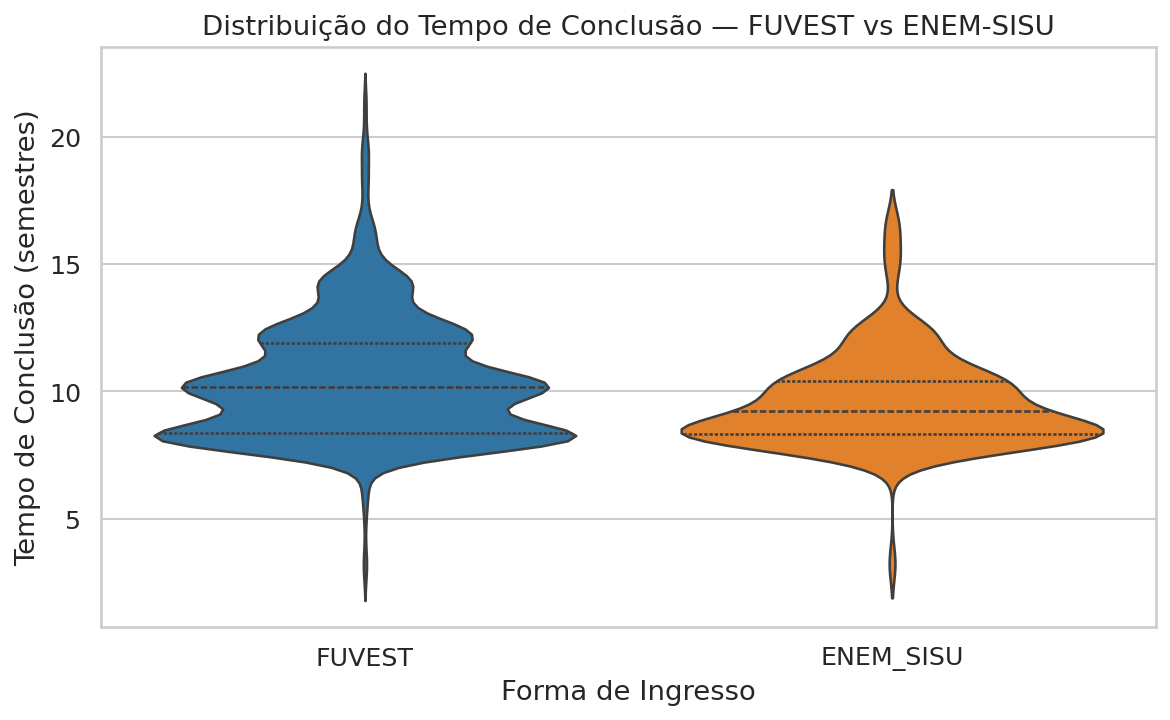
\includegraphics[width=0.75\textwidth]{figuras/fig9_violin_conclusao.png}
  \caption{Distribuição do tempo de conclusão (em semestres) para FUVEST e
  ENEM\_SISU. As linhas internas representam os quartis.}
  \label{fig:violin_conclusao}
\end{figure}

\subsubsection{Tempo até Evasão}

Alunos do ENEM\_SISU que evadiram saíram mais cedo do curso (mediana de
\textbf{5,3 semestres}) em comparação aos alunos do FUVEST (mediana de
\textbf{7,3 semestres}), sugerindo maior vulnerabilidade precoce nesse grupo.

\subsection{Créditos Acumulados}

A Figura~\ref{fig:hist_cr} mostra as distribuições de créditos acumulados para
alunos que concluíram e que evadiram. A diferença é marcante: quem concluiu
acumulou em mediana \textbf{188 créditos}, enquanto quem evadiu acumulou
apenas \textbf{38 créditos} — refletindo o abandono precoce de grande
parcela dos evadidos.

\begin{figure}[H]
  \centering
  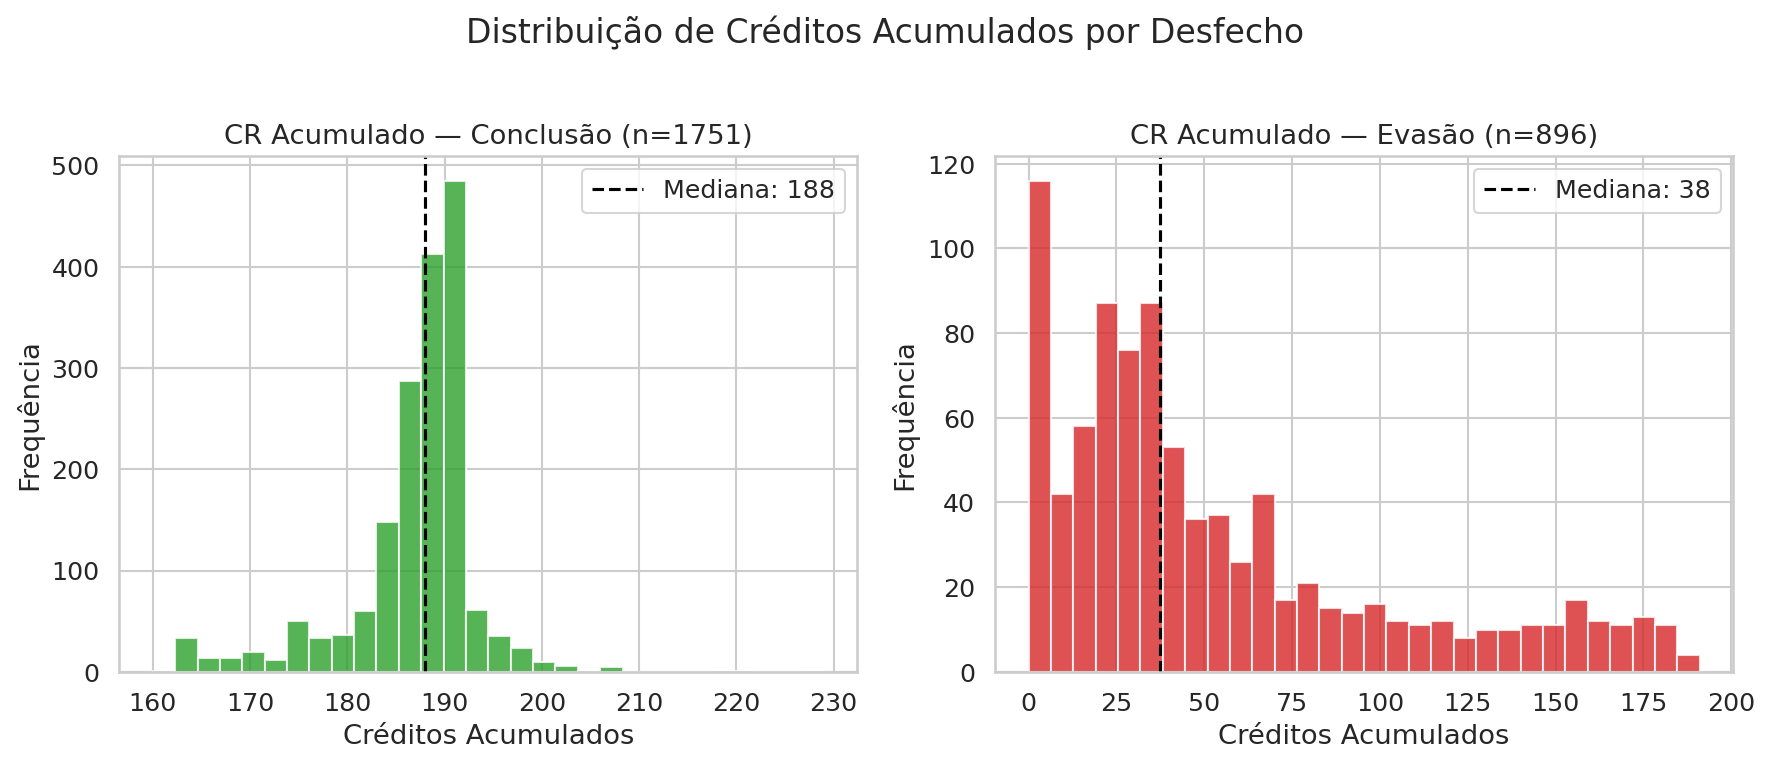
\includegraphics[width=0.95\textwidth]{figuras/fig4_hist_cr.png}
  \caption{Distribuição de créditos acumulados por desfecho. A linha
  tracejada indica a mediana de cada grupo.}
  \label{fig:hist_cr}
\end{figure}

\subsection{Evasão Precoce vs.\ Tardia}

Definiu-se evasão \textbf{precoce} como aquela ocorrida antes de 4 semestres
de curso. A Figura~\ref{fig:evasao_precoce} mostra que a evasão precoce é mais
pronunciada no grupo ENEM\_SISU: \textbf{46\%} dos alunos desse grupo que
evadiram o fizeram nos primeiros 4 semestres, contra \textbf{33\%} no FUVEST.

\begin{figure}[H]
  \centering
  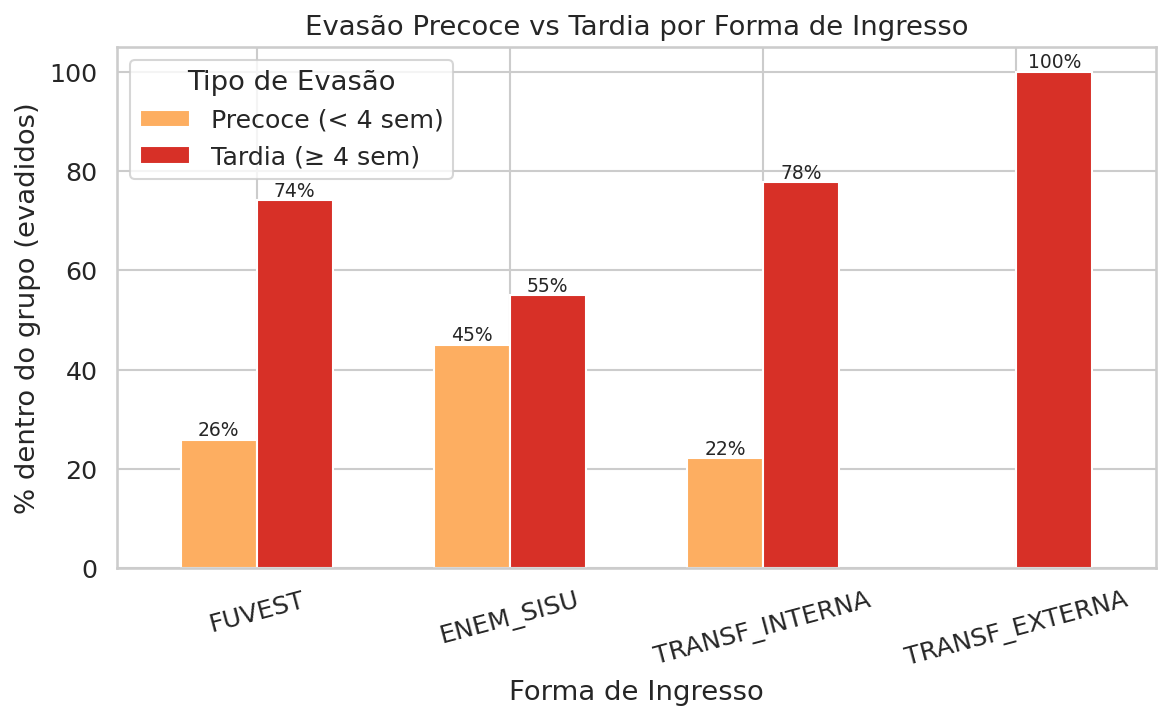
\includegraphics[width=0.75\textwidth]{figuras/fig10_evasao_precoce_tardia.png}
  \caption{Proporção de evasão precoce ($< 4$ semestres) e tardia ($\geq 4$
  semestres) por forma de ingresso, calculada dentro do subconjunto de
  evadidos.}
  \label{fig:evasao_precoce}
\end{figure}

\subsection{Evolução Temporal por Coorte}

A Figura~\ref{fig:evolucao_temporal} apresenta a evolução das taxas de evasão
e conclusão para todas as coortes de ingresso entre 2005 e 2021. Observa-se
uma tendência de redução da evasão e aumento da conclusão nas coortes mais
recentes (especialmente a partir de 2018), que pode estar associada tanto a
mudanças no perfil do curso quanto a um efeito de truncamento — coortes mais
recentes tiveram menos tempo para atingir o limite de prazo.

\begin{figure}[H]
  \centering
  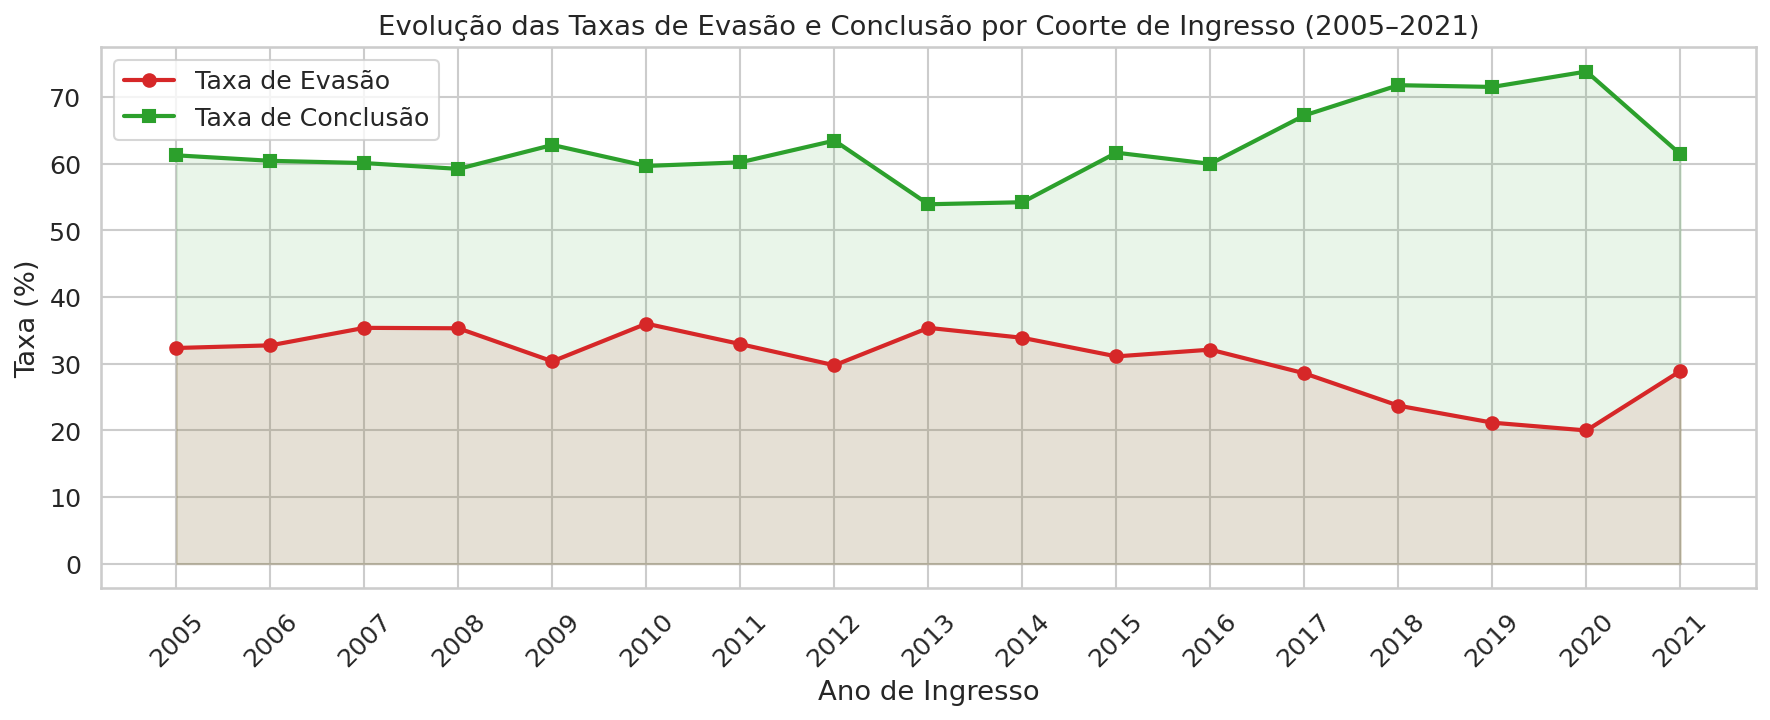
\includegraphics[width=0.95\textwidth]{figuras/fig5_evolucao_temporal.png}
  \caption{Evolução das taxas de evasão e conclusão por coorte de ingresso
  (2005--2021). Coortes de 2022 em diante foram excluídas por baixo volume
  de registros.}
  \label{fig:evolucao_temporal}
\end{figure}

A Figura~\ref{fig:heatmap} apresenta um \emph{heatmap} da taxa de evasão por
coorte e forma de ingresso, e a Figura~\ref{fig:evolucao_fuvest_enem}
compara diretamente as trajetórias de FUVEST e ENEM\_SISU por coorte.

\begin{figure}[H]
  \centering
  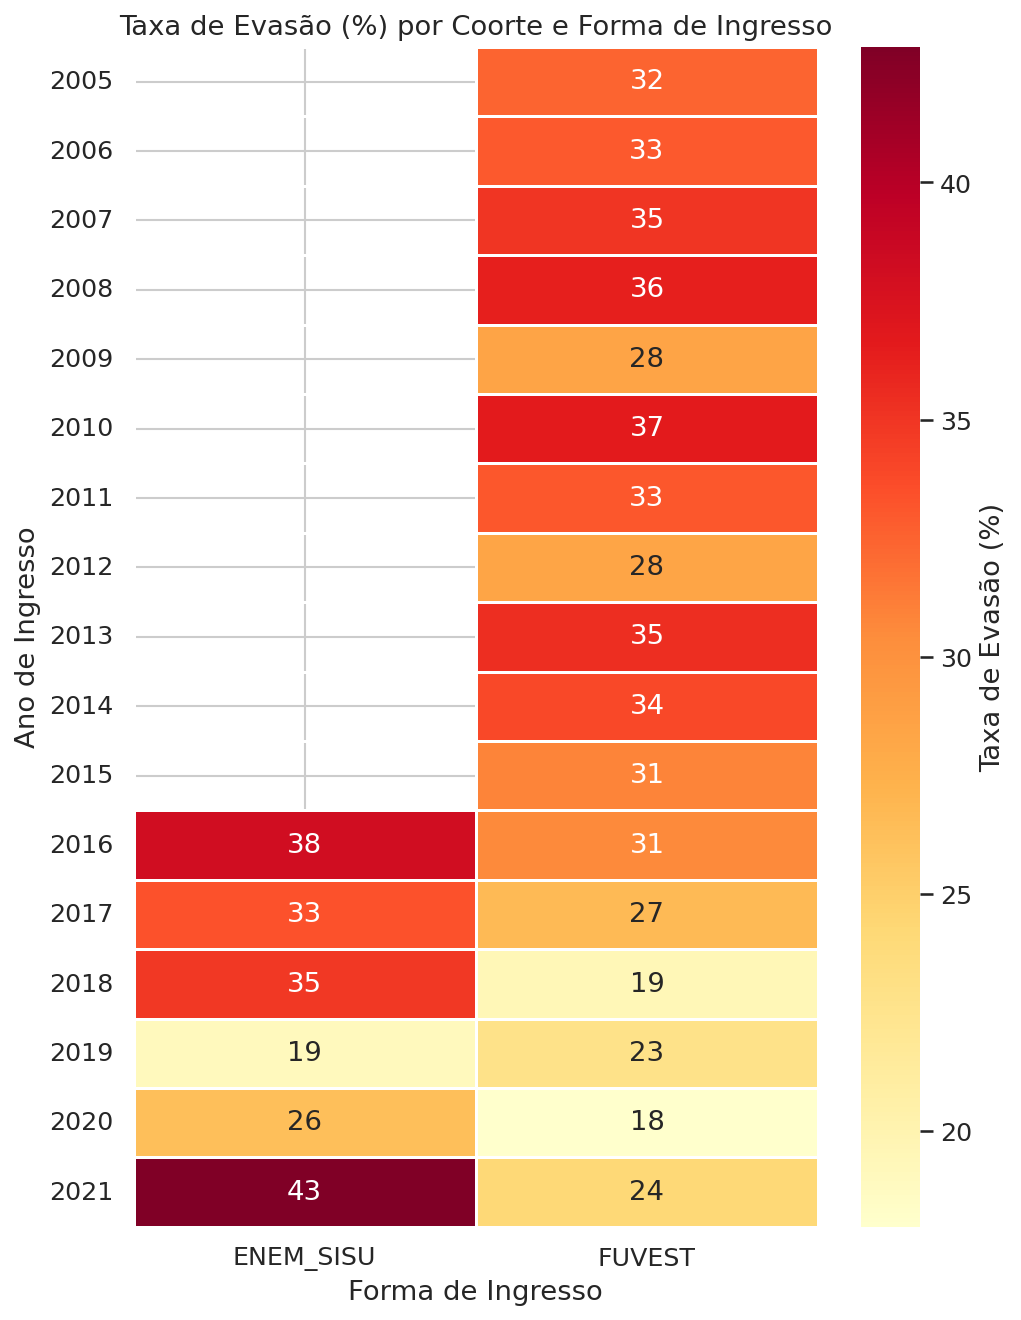
\includegraphics[width=0.55\textwidth]{figuras/fig6_heatmap_coorte.png}
  \caption{\emph{Heatmap} da taxa de evasão (\%) por coorte de ingresso e
  forma de ingresso. Células em branco indicam ausência de alunos
  daquela combinação naquele ano.}
  \label{fig:heatmap}
\end{figure}

\begin{figure}[H]
  \centering
  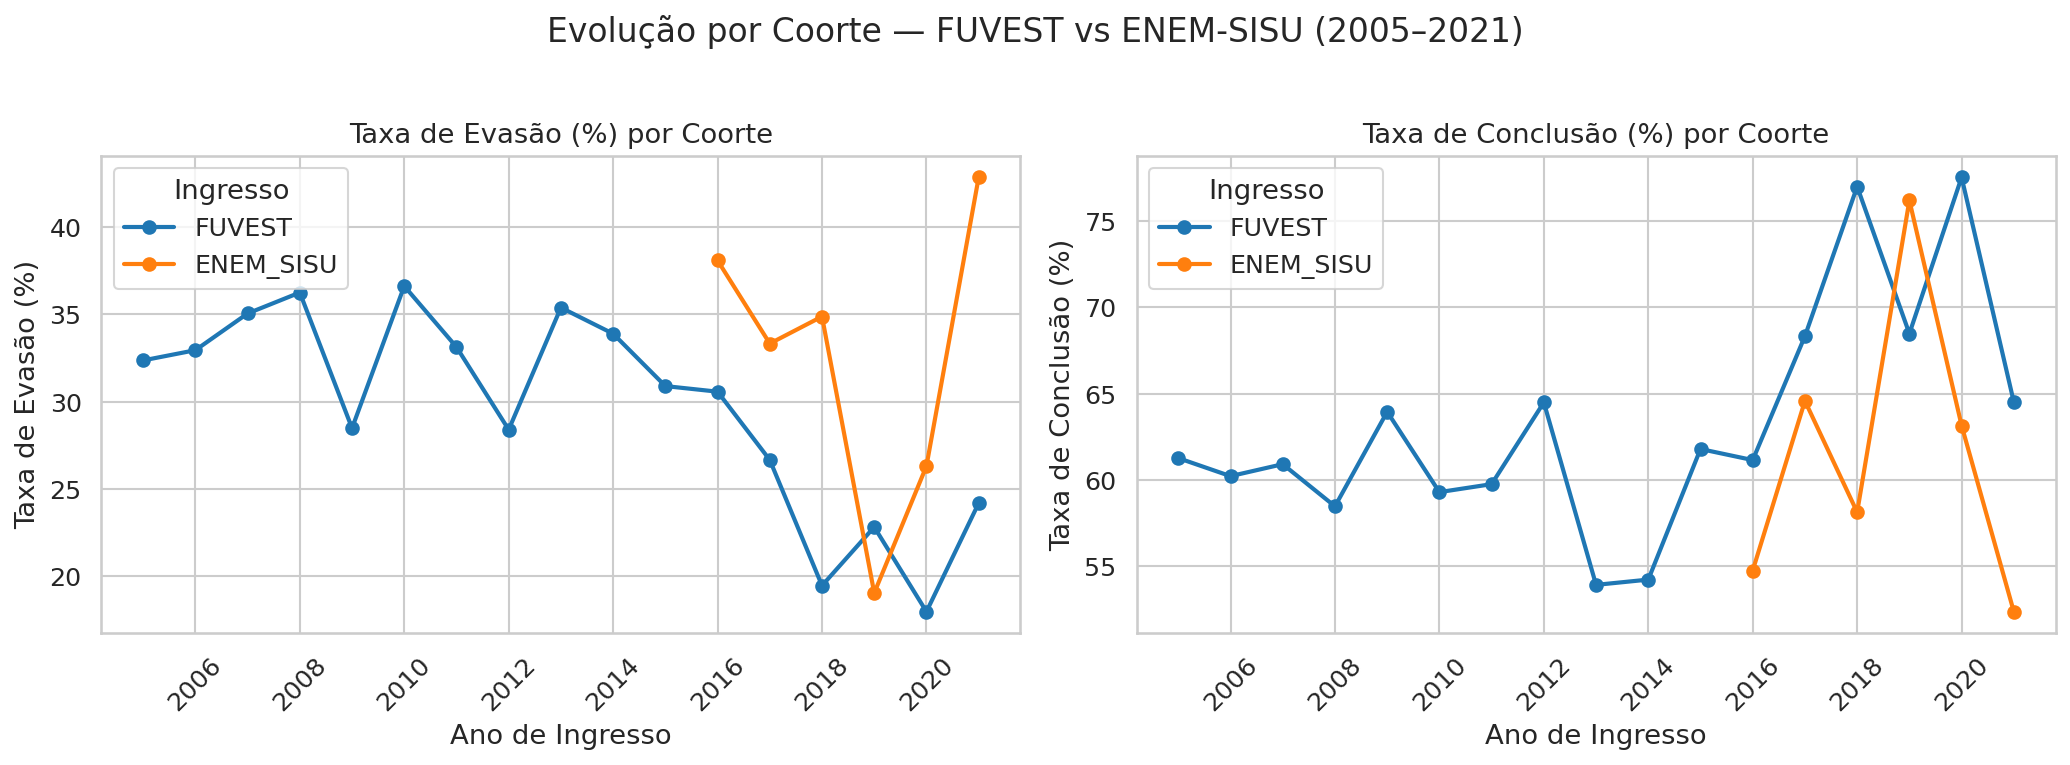
\includegraphics[width=0.95\textwidth]{figuras/fig8_evolucao_fuvest_enem.png}
  \caption{Evolução das taxas de evasão (esquerda) e conclusão (direita) por
  coorte de ingresso, comparando FUVEST e ENEM\_SISU (2016--2021 para
  ENEM\_SISU, que iniciou em 2016).}
  \label{fig:evolucao_fuvest_enem}
\end{figure}

% =============================================================================
\section{Análise Estatística}
% =============================================================================

\subsection{Análise de Sobrevivência — Kaplan-Meier}

A Figura~\ref{fig:km} apresenta as curvas de Kaplan-Meier para os grupos
FUVEST e ENEM\_SISU. O eixo vertical representa a probabilidade de o aluno
não ter evadido até aquele semestre (\emph{sobrevivência}).

\begin{figure}[H]
  \centering
  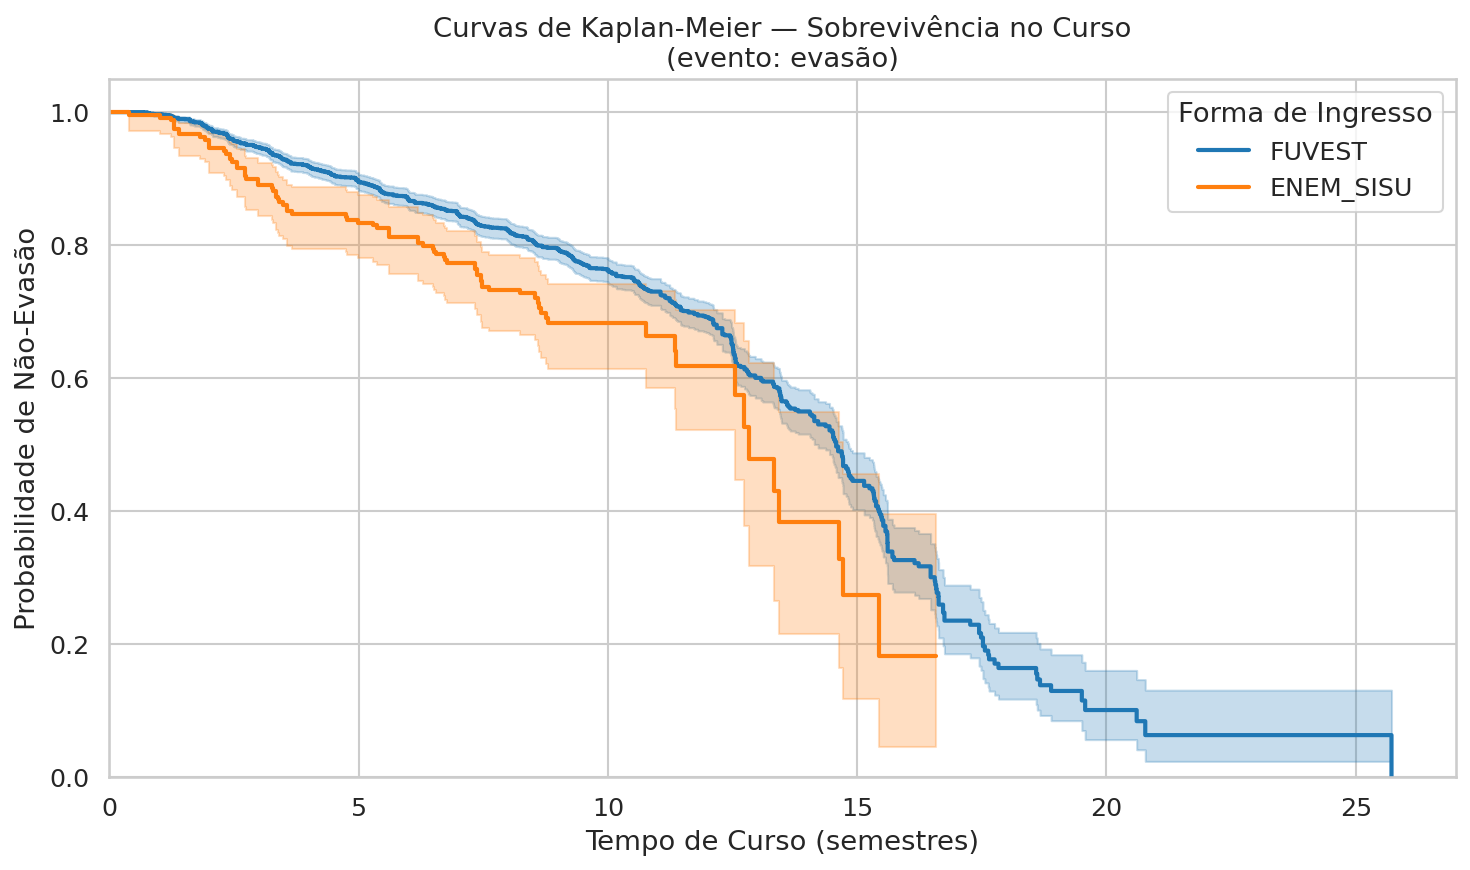
\includegraphics[width=0.88\textwidth]{figuras/fig7_kaplan_meier.png}
  \caption{Curvas de Kaplan-Meier — probabilidade de não-evasão ao longo do
  curso. As faixas sombreadas representam os intervalos de confiança de 95\%.
  Evento: evasão. Censurado: conclusão, transferência, reingresso.}
  \label{fig:km}
\end{figure}

A mediana de sobrevivência (semestre a partir do qual 50\% dos alunos
já teriam evadido, caso seguissem a mesma tendência) foi de
\textbf{14,6 semestres para FUVEST} e \textbf{12,8 semestres para ENEM\_SISU}.
O \textbf{teste log-rank} rejeitou a hipótese de igualdade das curvas
($\chi^2 = 10,04$; $p = 0{,}0015$), indicando diferença estatisticamente
significativa no padrão temporal de evasão entre os dois grupos.

\subsection{Testes de Hipóteses}

Os resultados dos testes inferenciais são apresentados na
Tabela~\ref{tab:testes}.

\begin{table}[H]
\centering
\caption{Resultados dos testes estatísticos}
\label{tab:testes}
\begin{tabular}{@{}llccc@{}}
\toprule
\textbf{Teste} & \textbf{Comparação} & \textbf{Estatística} & \textbf{p-valor} & \textbf{Conclusão} \\
\midrule
$\chi^2$ & Taxa de evasão: FUVEST vs ENEM\_SISU    & 0,326  & 0,569 & Não rejeita $H_0$ \\
$\chi^2$ & Taxa de conclusão: FUVEST vs ENEM\_SISU & 0,060  & 0,806 & Não rejeita $H_0$ \\
Mann-Whitney $U$ & Tempo de conclusão                & 134.040 & 0,0003 & Rejeita $H_0$ \\
Mann-Whitney $U$ & Tempo até evasão                  & 39.957 & 0,0001 & Rejeita $H_0$ \\
Mann-Whitney $U$ & CR acumulado: Conclusão vs Evasão & 1.560.938 & $<0,001$ & Rejeita $H_0$ \\
Log-rank         & Curvas KM: FUVEST vs ENEM\_SISU   & 10,040 & 0,0015 & Rejeita $H_0$ \\
\bottomrule
\end{tabular}
\end{table}

Os testes qui-quadrado indicam que as \textbf{taxas absolutas de evasão e
conclusão não diferem significativamente} entre FUVEST e ENEM\_SISU.
Contudo, os testes de Mann-Whitney revelam que o \textbf{tempo até esses
eventos é significativamente diferente}: alunos do ENEM\_SISU concluem mais
rápido (mediana 9,2 vs.\ 10,2 semestres) e, entre os que evadem, o fazem
mais cedo (mediana 5,3 vs.\ 7,3 semestres). O teste log-rank confirma essa
diferença no padrão temporal via análise de sobrevivência.

\subsection{Regressão Logística}

O modelo de regressão logística ajustado para predizer evasão (vs.\
conclusão) a partir de ingresso (ENEM\_SISU = 1), tempo de curso e créditos
acumulados obteve AUC de \textbf{0,998} ($\pm 0,002$) em validação cruzada
de 5 dobras, indicando excelente capacidade discriminativa.

Os coeficientes padronizados (Tabela~\ref{tab:regressao}) revelam que
\textbf{créditos acumulados é o preditor de maior magnitude} (coef.
$= -8{,}57$, sinal negativo: mais créditos $\to$ menor chance de evasão),
seguido pelo tempo de curso (coef. $= 1{,}58$). A forma de ingresso
(ENEM\_SISU) apresenta coeficiente negativo ($-0{,}27$), sugerindo
ligeiramente menor probabilidade de evasão para esse grupo quando controlados
os demais fatores — embora o efeito seja de pequena magnitude.

\begin{table}[H]
\centering
\caption{Coeficientes padronizados do modelo de regressão logística}
\label{tab:regressao}
\begin{tabular}{@{}lc@{}}
\toprule
\textbf{Preditor} & \textbf{Coeficiente padronizado} \\
\midrule
Ingresso (ENEM\_SISU = 1)  & $-0{,}2745$ \\
Tempo no curso (semestres) & $+1{,}5761$  \\
Créditos acumulados        & $-8{,}5654$  \\
\bottomrule
\end{tabular}
\end{table}

\textbf{Nota:} os preditores tempo de curso e créditos acumulados são
parcialmente endógenos ao desfecho (um aluno que evadiu cedo naturalmente
tem menos tempo e créditos). O modelo deve ser interpretado como uma
quantificação das associações, e não como um modelo causal.

% =============================================================================
\section{Discussão}
% =============================================================================

Os resultados deste estudo revelam um panorama nuançado sobre os padrões de
conclusão e evasão no curso de Sistemas de Informação da EACH-USP.

\textbf{Taxas gerais.} A taxa de conclusão de 61,5\% está em linha com a
média nacional de cursos de graduação públicos, e a taxa de evasão de 31,4\%,
embora expressiva, é consistente com o que a literatura reporta para cursos
tecnológicos \citep{silva_filho2007}.

\textbf{Comparação FUVEST vs.\ ENEM\_SISU.} A ausência de diferença
significativa nas taxas absolutas de evasão e conclusão ($p > 0{,}5$)
é um resultado relevante: alunos ingressantes pelo ENEM/SISU concluem e
evadem em proporções semelhantes aos do FUVEST. Isso contraria narrativas
que associam o ingresso por ENEM a piores resultados acadêmicos.

Contudo, o \textbf{padrão temporal} difere: alunos do ENEM\_SISU concluem
em menos tempo (9,2 vs.\ 10,2 semestres, $p < 0{,}001$) e, entre os
evadidos, saem mais cedo (5,3 vs.\ 7,3 semestres, $p < 0{,}001$). A maior
proporção de evasão precoce no ENEM\_SISU (46\% nos primeiros 4 semestres)
sugere que esses alunos podem enfrentar maior choque de adaptação nos
primeiros semestres.

\textbf{Motivos de evasão.} O cancelamento por créditos insuficientes
(43\% das evasões) e o trancamento sem reingresso (22,5\%) são os motivos
dominantes, sugerindo que parte significativa da evasão é de natureza
\emph{passiva} — o aluno vai perdendo o vínculo gradualmente, em vez de
formalizar uma desistência.

\textbf{Evolução temporal.} A redução nas taxas de evasão nas coortes mais
recentes (2018--2021) é promissora, mas deve ser interpretada com cautela:
alunos com menos tempo de curso têm menos oportunidade de atingir os
mecanismos de cancelamento por prazo, podendo haver um efeito de
\emph{left truncation} nas coortes recentes.

\textbf{Limitações.} Este estudo apresenta as seguintes limitações: (i) a
base não contém variáveis socioeconômicas, que são reconhecidamente
associadas à evasão; (ii) não há dados de empregabilidade dos egressos;
(iii) os grupos ENEM\_USP, OLIMP, GRADUADO, CONV\_PEC\_G e transferências
têm amostras muito pequenas, impedindo análises inferenciais robustas.

% =============================================================================
\section{Conclusão}
% =============================================================================

Este estudo analisou 2.849 históricos de alunos com vínculo encerrado no
curso de Sistemas de Informação da EACH-USP, abrangendo duas décadas de
funcionamento do curso. Os principais achados são:

\begin{enumerate}
  \item A taxa de conclusão (61,5\%) e evasão (31,4\%) do curso são
    comparáveis à média nacional para cursos tecnológicos.
  \item Alunos ingressantes pelo \textbf{FUVEST e ENEM\_SISU apresentam taxas
    absolutas de evasão e conclusão estatisticamente indistinguíveis}
    ($\chi^2$, $p > 0{,}5$).
  \item Alunos do \textbf{ENEM\_SISU concluem mais rapidamente} (mediana de
    9,2 semestres vs.\ 10,2 para FUVEST) e, quando evadem,
    \textbf{o fazem mais cedo} (mediana 5,3 vs.\ 7,3 semestres),
    conforme confirmado pelo teste de Mann-Whitney e pelas curvas de
    Kaplan-Meier (log-rank: $p = 0{,}0015$).
  \item O principal motivo de evasão é o cancelamento administrativo por
    insuficiência de créditos (43\%), indicando abandono gradual.
  \item O modelo de regressão logística identifica os créditos acumulados
    como principal preditor de desfecho, reforçando que o progresso acadêmico
    precoce é um fator protetor contra a evasão.
\end{enumerate}

Os resultados oferecem subsídios para o desenvolvimento de políticas de
permanência, especialmente voltadas ao \textbf{acompanhamento dos primeiros
semestres} — período crítico para ambos os grupos, mas especialmente para
alunos do ENEM\_SISU. Estudos futuros deveriam incorporar dados
socioeconômicos, desempenho por disciplina e variáveis de engajamento
institucional para aprofundar a compreensão dos determinantes da evasão.

% =============================================================================
\section*{Apêndice: Código Python da Análise}
\addcontentsline{toc}{section}{Apêndice: Código Python da Análise}
% =============================================================================

Esta seção apresenta os trechos principais do código utilizado na análise.
O script completo está disponível no arquivo \texttt{analise.py}.

\subsection*{Carga e pré-processamento}

\begin{lstlisting}[style=python, caption={Carga, conversão de datas e classificação de desfechos}]
import pandas as pd
import numpy as np

df = pd.read_excel('BASE_ALUNOS_FINAL.xlsx')

# Converter tempo de dias para semestres
df['TEMPO_SEMESTRES'] = df['TEMPO_CURSO'] / 180
df['ANO_INGRESSO'] = df['DATA_INGRESSO'].dt.year

# Classificar desfechos
EVASAO       = {'ABANDONO_FREQUENCIA','ABANDONO_MATRICULA','CANC_CREDITO',
                'CANC_VENCIMENTO','DESISTENCIA','TRANCAMENTO'}
CONCLUSAO    = {'CONCLUSAO'}
CONTINUA_USP = {'REINGRESSO','TRANSF_INT'}
SAIDA_EXT    = {'TRANSF_EXT','CANC_OUTRA_IES'}

def classificar_desfecho(te):
    if te in CONCLUSAO:    return 'Conclusao'
    if te in EVASAO:       return 'Evasao'
    if te in CONTINUA_USP: return 'Continua na USP'
    if te in SAIDA_EXT:    return 'Saida para outra IES'
    return 'Outros'

df['DESFECHO'] = df['TIPO_ENCERRAMENTO'].apply(classificar_desfecho)
df['EVADIU']   = (df['DESFECHO'] == 'Evasao').astype(int)
\end{lstlisting}

\subsection*{Análise de sobrevivência — Kaplan-Meier}

\begin{lstlisting}[style=python, caption={Estimação das curvas de Kaplan-Meier e teste log-rank}]
from lifelines import KaplanMeierFitter
from lifelines.statistics import logrank_test

grupos = ['FUVEST', 'ENEM_SISU']
kmfs = {}

fig, ax = plt.subplots(figsize=(10, 6))
for grupo in grupos:
    sub = df[df['TIPO_INGRESSO'] == grupo]
    kmf = KaplanMeierFitter()
    kmf.fit(sub['TEMPO_SEMESTRES'],
            event_observed=sub['EVADIU'],
            label=grupo)
    kmf.plot_survival_function(ax=ax, ci_show=True)
    kmfs[grupo] = (sub['TEMPO_SEMESTRES'], sub['EVADIU'])

# Teste log-rank
T1, E1 = kmfs['FUVEST']
T2, E2 = kmfs['ENEM_SISU']
resultado = logrank_test(T1, T2,
                         event_observed_A=E1,
                         event_observed_B=E2)
print(f"p-valor log-rank: {resultado.p_value:.4f}")
\end{lstlisting}

\subsection*{Testes de hipóteses}

\begin{lstlisting}[style=python, caption={Qui-quadrado e Mann-Whitney}]
from scipy.stats import chi2_contingency, mannwhitneyu

# Qui-quadrado: evasao vs nao-evasao por ingresso
ct = pd.crosstab(df['TIPO_INGRESSO'],
                 df['DESFECHO'].apply(
                     lambda x: 'Evasao' if x == 'Evasao' else 'Nao-Evasao'))
chi2, p, dof, _ = chi2_contingency(ct)
print(f"chi2={chi2:.4f}, p={p:.4f}")

# Mann-Whitney: tempo de conclusao por ingresso
t_fuv = df[(df['TIPO_INGRESSO']=='FUVEST') &
           (df['DESFECHO']=='Conclusao')]['TEMPO_SEMESTRES']
t_ene = df[(df['TIPO_INGRESSO']=='ENEM_SISU') &
           (df['DESFECHO']=='Conclusao')]['TEMPO_SEMESTRES']
u, p_mw = mannwhitneyu(t_fuv, t_ene, alternative='two-sided')
print(f"U={u:.0f}, p={p_mw:.4f}")
\end{lstlisting}

\subsection*{Regressão logística}

\begin{lstlisting}[style=python, caption={Regressão logística com validação cruzada}]
from sklearn.linear_model import LogisticRegression
from sklearn.preprocessing import StandardScaler
from sklearn.model_selection import cross_val_score

df_reg = df[df['TIPO_INGRESSO'].isin(['FUVEST','ENEM_SISU']) &
            df['DESFECHO'].isin(['Conclusao','Evasao'])].copy()
df_reg['ING_BIN'] = (df_reg['TIPO_INGRESSO'] == 'ENEM_SISU').astype(int)

X = df_reg[['ING_BIN','TEMPO_SEMESTRES','CR_ACUMULADO']].values
y = df_reg['EVADIU'].values

scaler = StandardScaler()
X_sc   = scaler.fit_transform(X)

modelo = LogisticRegression(max_iter=500)
auc    = cross_val_score(modelo, X_sc, y, cv=5, scoring='roc_auc')
print(f"AUC: {auc.mean():.3f} +/- {auc.std():.3f}")
\end{lstlisting}

% =============================================================================
% Referências
% =============================================================================
\bibliographystyle{plainnat}
\begin{thebibliography}{99}

\bibitem[Baggi e Lopes(2011)]{baggi2011}
Baggi, C. A. S., \& Lopes, D. A. (2011).
Evasão e avaliação institucional no ensino superior: uma discussão bibliográfica.
\textit{Avaliação}, 16(2), 355--374.

\bibitem[Borges et al.(2020)]{borges2020}
Borges, F. T., Aquino, C. A. B., \& Puente-Palacios, K. (2020).
Análise de sobrevivência aplicada ao estudo da evasão universitária.
\textit{Estudos em Avaliação Educacional}, 31(78), 680--712.

\bibitem[Felicetti e Morosini(2014)]{felicetti2014}
Felicetti, V. L., \& Morosini, M. C. (2014).
Do compromisso e implicação discentes: um estudo em cursos de licenciatura.
\textit{Educar em Revista}, (51), 241--255.

\bibitem[Kaplan e Meier(1958)]{kaplan1958}
Kaplan, E. L., \& Meier, P. (1958).
Nonparametric estimation from incomplete observations.
\textit{Journal of the American Statistical Association}, 53(282), 457--481.

\bibitem[Mantel(1966)]{mantel1966}
Mantel, N. (1966).
Evaluation of survival data and two new rank order statistics arising in its consideration.
\textit{Cancer Chemotherapy Reports}, 50(3), 163--170.

\bibitem[Silva Filho et al.(2007)]{silva_filho2007}
Silva Filho, R. L. L., Motejunas, P. R., Hipólito, O., \& Lobo, M. B. C. M. (2007).
A evasão no ensino superior brasileiro.
\textit{Cadernos de Pesquisa}, 37(132), 641--659.

\bibitem[Tinto(1975)]{tinto1975}
Tinto, V. (1975).
Dropout from higher education: A theoretical synthesis of recent research.
\textit{Review of Educational Research}, 45(1), 89--125.

\bibitem[Vasconcelos et al.(2019)]{vasconcelos2019}
Vasconcelos, I. C. O., Lima, D. A., \& Araújo, M. A. D. (2019).
Democratização do acesso ao ensino superior e permanência estudantil:
análise das políticas de ação afirmativa no Brasil.
\textit{Ensaio: Avaliação e Políticas Públicas em Educação}, 27(104), 692--715.

\end{thebibliography}

\end{document}
